\section{ICT Abatement Potential and Rebound Effects}

\subsection{Abatement through ICT}

\begin{table}[h]
    \begin{tabular}{| c | l | l | l |}
    \hline
    \textbf{Sector} & \textbf{\makecell[l]{Substitution, \\ Dematerialization}} & \textbf{Increased Efficiency} & \textbf{\makecell[l]{Awareness and \\ decision support}} \\ \hline
    Transportation &
    \makecell[l]{Telepresence,\\Telework,\\Virtual conferences} &
    \makecell[l]{Route optimization} &
    \makecell[l]{Mobility footprint \\monitoring, \\Real time navigation}\\ \hline
    Households &
    E-shopping &
    Smart heating &
    \makecell[l]{In-home displayes,\\Normative feedback} \\ \hline
    Industry &
    \makecell[l]{3D printing,\\Virtual goods} &
    \makecell[l]{Smart heating,\\Smart logistics,\\Robots,\\AI-based automation} &
    \makecell[l]{Integrated supply chain} \\ \hline
    Energy &
    (Renewable integration) &
    \makecell[l]{Automatic demand \\response} &
    \makecell[l]{User based \\demand response,\\Gas leakage discovery} \\ \hline
    \end{tabular}

    \caption{Abatement potential of ICT in different sectors}
\end{table}

\subsection{The Rebound Effect}
The typical process of the rebound effect is as follows

\begin{enumerate}
    \item Baseline consumption
    \item Efficiency increase
    \item Product is more efficient, but also cheaper
    \item Increased consumption
\end{enumerate}

\begin{tcolorbox}
    \textbf{A Neoclassical Economics Perspective}\\

        \begin{center}
        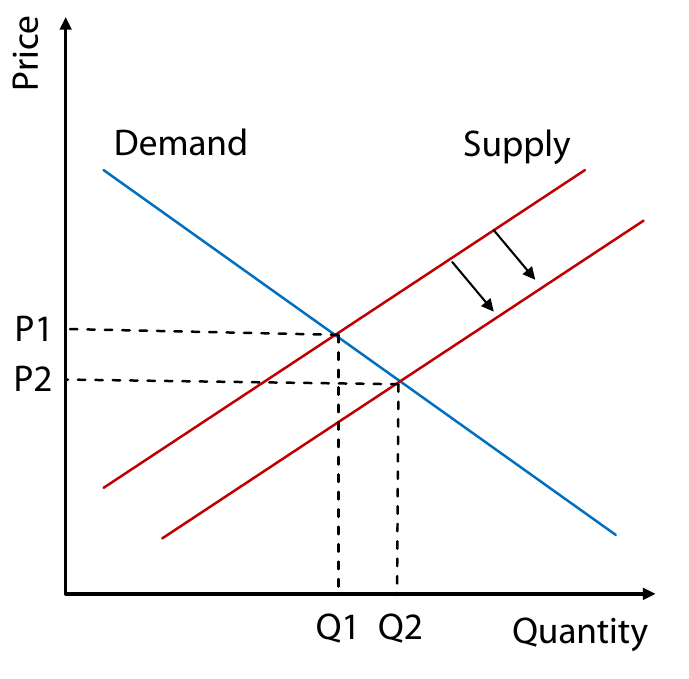
\includegraphics[width=0.50\linewidth]{rebound_market}
        \captionof{figure}{Market equilbrium before and after efficiency increase}\
        \label{fig:rebound_market}
        \end{center}

    Figure \ref{fig:rebound_market} shows the relationship between price, quantity, demand and supply.
    The market equilibrium maximizes the output.
    As efficiency increases, the producer's costs decreases.
    This pushes the supply curve down and a new equilibrium is reached.
    In this new equilibrium the prize is lower and the output higher.
\end{tcolorbox}

\subsubsection{Direct Rebound Effect}
Direct rebound is the counterbalance of the same good for which efficiency increased.
The direct rebound is typically expressed as a percentage.
An example from the transport sector is cars getting more efficient, leading to lower running costs and therefore people drive further and more often.

\subsubsection{Indirect Rebound Effect}
People do not spend their income on just one good, but rather on a whole set of goods.
Efficiency increase of one and the following price decrease rebalances what can be spent on different goods.
One good getting cheaper can thereby result in increased consumption of some other good.
Consider for example again the case of more efficient cars.
Instead of simply driving more the money saved could be used to travel more, paying for more flights.

\subsubsection{Limits of Rebound Effect}
Not all goods are affected by rebound effects.
Consider goods where a lower price does not particularly increase consumption (for example vacuum cleaners).
Also in cases where the energy is a minor cost component an increased energy efficiency doesn't affect the price much and therefore no rebound effect is observed.
It is also worth considering that not all increased consumption is negative.
For example increased use of train rides substituting some car rides would be beneficial from a sustainability viewpoint.\\

\begin{tcolorbox}
    \textbf{The Kaya Identity}\\
    The following relationship describes factors that affect \cotwo emissions.\\

    \begin{tabular}{ccccccccc}
        Emissions &
        $=$ &
        Population &
        $\cdot$ &
        Affluence &
        $\cdot$ &
        Energy Intensity &
        $\cdot$ &
        Carbon Intensity
        \\
        $\frac{\text{Gt\cotwo}}{year}$ & &
        Persons & &
        $\frac{\text{\$} / \text{person}}{\text{year}}$ & &
        $\frac{\text{kWh}}{\text{\$}} $ & &
        $\frac{\text{Gt\cotwo}}{\text{kWh}}$
    \end{tabular}

    \begin{itemize}
        \item Population will grow.
        \item De-growth proponements aim at limiting affluence.
        \item ICT can mainly contribute to decreasing energy intensity.
        \item ICT also has a central role in transition to zero carbon technology to decrease carbon intesity.
        \item In the EU the carbon intensity is decreasing.
    \end{itemize}
\end{tcolorbox}




